\documentclass[12pt,a4paper,titlepage]{article}
\usepackage[utf8]{inputenc}
\usepackage[finnish]{babel}
\usepackage{setspace}
\usepackage{parskip}
\usepackage{amssymb}
\usepackage{amsmath}
\usepackage{graphicx}
\usepackage{fancyhdr}
\usepackage[top=1in, bottom=1in, left=1in, right=1in]{geometry}
\usepackage{float}

%\usepackage[numbered,autolinebreaks,useliterate]{mcode} % jos tahdot laittaa matlabkoodia näkyville niin kannattaa käyttää tätä

% hyödyllisiä paketteja:
\usepackage{siunitx}\sisetup{per=frac} % SI-yksiköitä.
%\usepackage{supertabular} % jos tarttee isoja taulukoita
%\usepackage{fullpage} % pienemmät marginaalit jos haluaa

\usepackage{hyperref} % lisääthän omat pakettisi ENNEN hyperref'iä
\hypersetup{pdfborder={0 0 0}}
\onehalfspacing
\cfoot{}
\rhead{\thepage}
% asettaa nyk. kappaleen nimen vasempaan ylänurkkaan, saa poistaa jos haluaa
\lhead{\leftmark}

\usepackage{bm}
\newcommand{\matr}[1]{\bm{#1}}
\newcommand{\transpose}[1]{{#1}^T}
\newcommand{\var}{\text{var}}

%%%%% kaikki ennen tätä liittyy käytettäviin paketteihin tai dokumentin muotoiluun. siihen ei tarvinne aluksi koskea. %%%%%

%%%%% kansilehti %%%%%
\title{Taivaanmekaniikka \\ Lineaarinen pienimmän neliösumman sovitus \vspace{0.5em}}
\author{\begin{tabular}{c}
Anni Järvenpää
\end{tabular}}
\date{\today}
\begin{document}
\maketitle

\newpage
\null
\thispagestyle{empty}
\addtocounter{page}{-1}
\newpage

%%%%%%%%%%%%%%% Oleellinen sisältö alkaa%%%%%%%%%%%%%%%
\section{Lineaarinen pienimmän neliösumman menetelmä}
Lineaarisen pienimmän neliösumman menetelmän tavoitteena on sovittaa $n$ muotoa $(x_i, y_i)$ olevasta pisteestä koostuvaan havaintoaineistoon suora, joka edustaa pisteitä mahdollisimman hyvin. Tyypillisesti sovituksen hyvyyttä mitataan pisteiden vertikaalisena etäi\-syytenä~$|e|$ sovitetusta suorasta (merkitty sinisellä kuvassa \ref{vertikaalietaisyys}). Pienimmän neliösumman menetelmässä näiden vertikaalisten poikkeamien neliöiden summa pyritään minimoimaan, siis etsimään funktion $f(x) = \beta_1 + \beta_2 x + \beta_3 x^2 + ... + \beta_{m+1} x^m$ kertoimet $\beta_1 ... \beta_{m+1}$ siten, että virhe $S$ on mahdollisimman pieni, kun $S$ on määritelty yhtälön \ref{virhe} mukaisesti.~\cite{basicideas}
\begin{equation} \label{virhe}
	S = \sum\limits_{i=1}^{n} e_i^2 = \sum\limits_{i=1}^{n} (y_i - f(x_i))^2
\end{equation}

\begin{figure}
\centering
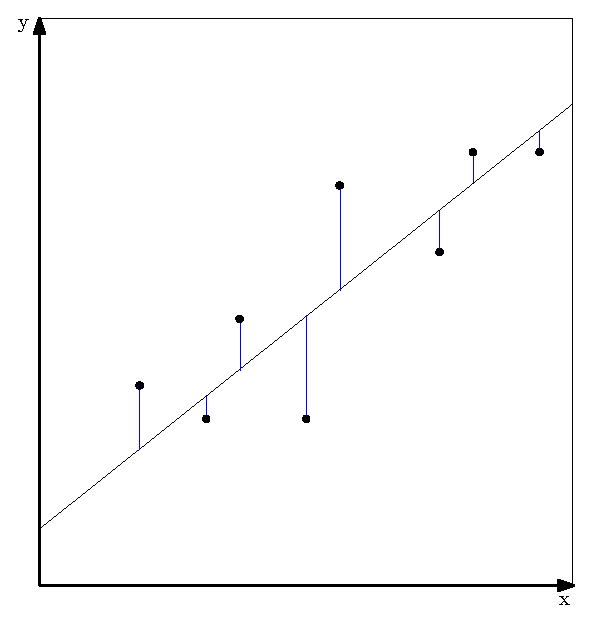
\includegraphics{vertikaalietaisyys.eps}
\caption{Pistejoukko, johon sovitettu suora mustalla ja pisteiden vertikaaliset etäisyydet suorasta pisteinä.}
\label{vertikaalietaisyys}
\end{figure}

Virheen minimiarvot löytyvät derivaatan nollakohdista:~\cite{wolframmath}
\begin{align*}
	\frac{\partial R^2}{\partial \beta_1} &= -2\sum\limits_{i=1}^n[y-(\beta_1+\beta_2x+...+\beta_{m+1}x^m)]=0 \\
	\frac{\partial R^2}{\partial \beta_2} &= -2\sum\limits_{i=1}^n[y-(\beta_1+\beta_2x+...+\beta_{m+1}x^m)]=0 \\
	&\vdots  \\
	\frac{\partial R^2}{\partial \beta_{m+1}} &= -2\sum\limits_{i=1}^n[y-(\beta_1+\beta_2x+...+\beta_{m+1}x^m)]=0
\end{align*}
Näistä saadaan edelleen 
\begin{align*}
	\beta_1 n+\beta_2\sum\limits_{i=1}^n x_i+...+\beta_{m+1} \sum\limits_{i=1}^n x_i^m &= \sum\limits_{i=1}^n y_i \\
	\beta_1\sum\limits_{i=1}^nx_i+\beta_1\sum\limits_{i=1}^nx_i^2+...+\beta_{m+1}\sum\limits_{i=1}^nx_i^{m+1} &= \sum\limits_{i=1}^n x_iy_i  \\
	\beta_1\sum\limits_{i=1}^nx_i^{m}+\beta_1\sum\limits_{i=1}^nx_i^{m+1}+...+\beta_{m+1}\sum\limits_{i=1}^nx_i^{2m} &= \sum\limits_{i=1}^n x_i^{m}y_i
\end{align*}
eli matriisimuodossa
\begin{equation} \label{matriisimuoto}
	\begin{bmatrix}
		n & \sum\limits_{i=1}^{n} x_i & ... & \sum\limits_{i=1}^{n} x_i^{m} \\
		\sum\limits_{i=1}^{n} x_i & \sum\limits_{i=1}^{n} x_i^2 & ... & \sum\limits_{i=1}^{n} x_i^{m+1} \\
		\vdots & \vdots & \ddots  & \vdots \\
		\sum\limits_{i=1}^{n} x_i^{m} & \sum\limits_{i=1}^{n} x_i^{m+1} & ... & \sum\limits_{i=1}^{n} x_i^{2m}
	\end{bmatrix}
	\begin{bmatrix}
		\beta_1 \\
		\beta_2 \\
		\vdots \\
		\beta_{m} \\
		\beta_{m+1} \\
	\end{bmatrix}
	=
	\begin{bmatrix}
		\sum\limits_{i=1}^n y_1 \\
		\sum\limits_{i=1}^n y_2 \\
		\vdots \\
		\sum\limits_{i=1}^n y_{m} \\
	\end{bmatrix}.
\end{equation}

Voidaan myös huomata, että yhtälöön \ref{matriisimuoto} voidaan päästä hyödyntämällä Vandermonden matriisia \cite{vandermonde}
\begin{equation}
	\matr{X} = 
	\begin{bmatrix}
		1 & x_{1}^2 & ...    & x_{1}^n \\
		1 & x_{2}^2 & ...    & x_{2}^n \\
		\vdots  & \vdots  & \ddots & \vdots  \\
		1 & x_{m}^2 &    ... & x_{m}^n
	\end{bmatrix}
\end{equation}
ja kirjoittamalla tämän avulla
\begin{equation} \label{matriiseilla}
	\begin{bmatrix}
			1 & x_{1} & x_{1}^2 & ...    & x_{1}^n \\
			1  & x_{2}& x_{2}^2 & ...    & x_{2}^n \\
			1  & x_{3}& x_{3}^2 & ...    & x_{3}^n \\
			\vdots  & \vdots  & \vdots & \ddots & \vdots  \\
			1  & x_{n}& x_{m}^2 &    ... & x_{m}^n
	\end{bmatrix}
	\begin{bmatrix}
		\beta_1 \\
		\beta_2 \\
		\vdots \\
		\beta_{m+1} \\
	\end{bmatrix}
	=
	\begin{bmatrix}
		y_1 \\
		y_2 \\
		\vdots \\
		y_n
	\end{bmatrix}.
\end{equation}
Nyt voidaan kertoa edellinen yhtälö puolittain vasemmalta Vandermonden matriisin transpoosilla $\transpose{\matr{X}}$, jolloin yhtälö saadaan seuraavaan muotoon:
\begin{equation*} 
	\begin{bmatrix}
		1       & 1       & 1 & ...    & 1 \\
		x_{1} & x_{2} &  x_3 &...    &  x_{m}\\
		x_{1}^2 & x_{2}^2 & x_3^3 & ...    &  x_{m}^2\\
		\vdots  & \vdots  & \vdots & \ddots & \vdots  \\
		x_{1}^n & x_{2}^n & x_3^n &   ... & x_{m}^n
	\end{bmatrix}
	\begin{bmatrix}
			1 & x_{1} & x_{1}^2 & ...    & x_{1}^n \\
			1  & x_{2}& x_{2}^2 & ...    & x_{2}^n \\
			1  & x_{3}& x_{3}^2 & ...    & x_{3}^n \\
			\vdots  & \vdots  & \vdots & \ddots & \vdots  \\
			1  & x_{n}& x_{m}^2 &    ... & x_{m}^n
	\end{bmatrix}
	\begin{bmatrix}
		\beta_1 \\
		\beta_2 \\
		\vdots \\
		\beta_{m+1} \\
	\end{bmatrix}
	=
	\begin{bmatrix}
		1       & 1       & ...    & 1 \\
		x_{1}^2 & x_{2}^2 & ...    &  x_{m}^2\\
		\vdots  & \vdots  & \ddots & \vdots  \\
		x_{1}^n & x_{2}^n &    ... & x_{m}^n
	\end{bmatrix}
	\begin{bmatrix}
		y_1 \\
		y_2 \\
		\vdots \\
		y_n
	\end{bmatrix}.
\end{equation*}
Suoritetaan yhtälön matriisien kertolaskut, jolloin saadaan
\begin{equation}\label{vandermondesta}
	\begin{bmatrix}
		n & \sum\limits_{i=1}^{n} x_i & ... & \sum\limits_{i=1}^{n} x_i^{m} \\
		\sum\limits_{i=1}^{n} x_i & \sum\limits_{i=1}^{n} x_i^2 & ... & \sum\limits_{i=1}^{n} x_i^{m+1} \\
		\vdots & \vdots & \ddots  & \vdots \\
		\sum\limits_{i=1}^{n} x_i^{m} & \sum\limits_{i=1}^{n} x_i^{m+1} & ... & \sum\limits_{i=1}^{n} x_i^{2m}
	\end{bmatrix}
	\begin{bmatrix}
		\beta_1 \\
		\beta_2 \\
		\vdots \\
		\beta_{m+1} \\
	\end{bmatrix}
	=
	\begin{bmatrix}
		\sum\limits_{i=1}^n y_1 \\
		\sum\limits_{i=1}^n y_2 \\
		\vdots \\
		\sum\limits_{i=1}^n y_{m} \\
	\end{bmatrix}.
\end{equation}
Nyt voidaan huomata yhtälöiden \ref{vandermondesta} ja \ref{matriisimuoto} olevan identtiset. Koska Vandermonden matriisi on kääntyvä\footnote{Mikä voidaan helposti osoittaa, ks. esim \url{https://proofwiki.org/wiki/Inverse_of_Vandermonde's_Matrix}}, on kaikille yhtälöstä \ref{matriiseilla} yhtälöön \ref{vandermondesta} pääsemiseksi tehdyille operaatioille käänteisoperaatio. Täten yhtälöt \ref{matriiseilla} ja \ref{matriisimuoto} ovat yhtäpitävät, eli pienimmän neliösumman antavat kertoimet $\beta_i$ voidaan ratkaista yhtälöstä \ref{matriiseilla}.

Otetaan kerroinvektorin ratkaisemisen helpottamiseksi käyttöön seuraavat merkinnät:
\begin{equation*}
	\matr{Y} =
		\begin{bmatrix}
			y_1 \\
			y_2 \\
			\vdots \\
			y_n
		\end{bmatrix} \quad \text{ja} \quad
	\matr{\beta} =
		\begin{bmatrix}
			\beta_1 \\
			\beta_2 \\
			\vdots \\
			\beta_m			
		\end{bmatrix},
\end{equation*}
jolloin yhtälö \ref{matriisimuoto} voidaan kirjoittaa lyhyesti
\begin{equation}
	\matr{Y} = \matr{X}\matr{\beta}
\end{equation}
ja tästä ratkaista $\matr{\beta}$ seuraavasti:
\begin{alignat}{2} \label{ilmanvirhetta}
	\matr{Y} &= \matr{X}\matr{\beta} &&|| \transpose{\matr{X}} \cdot \nonumber \\
	\transpose{\matr{X}}\matr{Y} &= \transpose{\matr{X}}\matr{X}\matr{\beta} &&|| (\transpose{\matr{X}}\matr{X}\matr{\beta})^{-1} \nonumber \\
	\matr{\beta} &= (\transpose{\matr{X}}\matr{X})^{-1}\transpose{\matr{X}}\matr{Y} \quad &&
\end{alignat}

Samankaltaisella päättelyketjulla voidaan ratkaista yleinen lauseke myös tilanteelle, jossa kaikkien pisteiden mittaustarkkuus ei ole sama, jolloin pisteille halutaan käyttää erilaisia painokertoimia sovitusta tehtäessä. Tähän voidaan käyttää varianssimatriisia $\matr{V}$, jonka avulla voidaan määritellä painokerroinmatriisi $\matr{W}=\matr{V}^{-1}\sigma^2$. Tässä $\sigma$ on tutkittavan aineiston varianssi ja $\matr{V}$ määritelty seuraavasti:~\cite{basicideas}
\begin{equation*}
	\matr{V}
	=
	\begin{bmatrix}
		\sigma_1^2   & \sigma_{1,2} &   ...  & \sigma_{1,n} \\
		\sigma_{2,1} & \sigma_2^2   &   ...  & \sigma_{2,n} \\
		\vdots       & \vdots       & \ddots & \vdots \\
		\sigma_{n,1}  & \sigma_{n,2}  &   ...  & \sigma_n^2
	\end{bmatrix}
\end{equation*}

Näitä merkintöjä käyttäen kerroinvektori $\matr{\beta}$ voidaan ratkaista yhtälöstä \ref{virheella}~\cite{basicideas}.
\begin{equation}\label{virheella}
	\matr{\beta} = (\transpose{\matr{X}}\matr{W}\matr{X})^{-1}\transpose{\matr{X}}\matr{W}\matr{Y}
\end{equation}

\section{Pienimmän neliösumman ratkaisu kaksiulotteiselle havaintoaineistolle} \label{2d}
Kun pienimmän neliösumman sovitusta sovelletaan asteroidin radanmääritykseen, on käytössä kaksiulotteinen havaintoaineisto, joka koostuu asteroidin paikoista $(x_i, y_i)$ ajanhetkillä $t_i$. Asteroidin paikkavektori $\matr{r}(t)$ mielivaltaisella ajanhetkellä $t$ voidaan ratkaista asteroidin rataelementtien avulla. Rataelementeiksi voidaan valita asteroidin paikka $\matr{R}_0 = (X_0, Y_0)$ ja nopeus $\matr{V}_0 = (\dot{X}_0, \dot{Y}_0)$ ajanhetkellä $t = 0$, jolloin asteroidin paikka saadaan seuraavasti:
\begin{equation} \label{r(t)}
	\matr{r}(t) = \matr{R}_0 + \matr{V}_0t.
\end{equation}	
	
Havaintoaineiston ollessa kaksiulotteinen, täytyy $\matr{Y}$-vektorin tallentaa sekä $x$- että $y$-koordinaatit, jolloin
\begin{equation*}
	\matr{Y}
	=
	\begin{bmatrix}
		x_1 \\
		y_2 \\
		x_2 \\
		y_2 \\
		\vdots \\
		x_n \\
		y_n
	\end{bmatrix}.
\end{equation*}
Koska tahdotaan ratkaista aiemmin määritellyt rataelementit, on myös ratkaistava kerroinvektori erilainen:
\begin{equation*}
	\matr{\beta}
	=
	\begin{bmatrix}
		X_0 \\
		Y_0 \\
		\dot{X}_0 \\
		\dot{Y}_0 \\
	\end{bmatrix}.
\end{equation*}
Myös havainnot sisältävän matriisin $\matr{X}$ täytyy mukautua kaksiulotteiseen havaintoaineistoon, jotta kertolasku $\matr{Y}$-vektorin kanssa on mahdollinen ja fysikaalisesti mielekäs. Tähän sopii alla esitetty matriisi, jolla $(\transpose{\matr{X}}\matr{X})^{-1}\transpose{\matr{X}}$ tuottaa
kooltaan $4 \times 2n$ matriisin, joka voidaan edelleen kertoa edellä määritellyllä vektorilla $\matr{Y}$, jolloin saadaan kooltaan matriisia $\matr{\beta}$ vastaava matriisi. Ajanhetki $t_i$ on pisteen $(x_i, y_i)$ havaintoaika.
\begin{equation*}
	\matr{X}
	=
	\begin{bmatrix}
		1 & 0 & t_1 & 0 \\
		0 & 1 & 0 & t_1 \\
		\vdots & \vdots & \vdots & \vdots \\
		1 & 0 & t_n & 0 \\
		0 & 1 & 0 & t_n
	\end{bmatrix} 
\end{equation*}

Näillä uudelleenmääritellyillä on mahdollista käyttää suoraan aiemmin ratkaistuja yhtälöitä \ref{ilmanvirhetta} (kaikkien havaintojen painokerroin sama) tai \ref{virheella} (painokertoimet). Mikäli käytetään painokertoimia, on myös painokerroinmatriisin koko luonnollisesti $2n~\times~2n$. Ratkaisuna saatavasta vektorista $\matr{\beta}$ saadaan suoraan rataelementit $\matr{R_0}$ ja $\matr{V_0}$.

\section{Ennusteen virhearvio lineaarisessa mallissa} \label{linvirhe}
Yhtälön \ref{virheella} mukaisesti ratkaistujen parametrien $\matr{\beta}$ virhe voidaan laskea kun tiedetään, että lineaarikombinaatiossa $\transpose{\matr{P}}\matr{Y}$, missä $\matr{P}$ on vakiovektori, saadaan varianssimatriisi seuraavasti \cite{basicideas}:
\begin{equation*}
	\text{var}(\transpose{\matr{P}}\matr{Y}) = \transpose{\matr{P}}\text{var}(\matr{Y})\matr{P}.
\end{equation*}
Tällöin saadaan
\begin{equation} \label{varianssihirvio}
	\var(\matr{\beta}) =  (\transpose{\matr{X}}\matr{W}\matr{X})^{-1}\transpose{\matr{X}}\matr{W}\var(\matr{\beta}) \matr{W}(\transpose{\matr{X}}\matr{W}\matr{X})^{-1}.
\end{equation}
Hyödyntämällä aiemmin määriteltyä $\matr{W}=\matr{V}^{-1}\sigma^2$ ja tietoa $\var(\matr{\beta})=\matr{V}$ eli $\var(\beta)~=~\sigma^2\matr{W}^{-1}$ saadaan yhtälö \ref{varianssihirvio} muotoon
\begin{equation}
	\var(\matr{\beta}) = \sigma^2(\transpose{\matr{X}}\matr{W}\matr{X})^{-1}	
\end{equation}

Kun parametrien $\beta_i$ varianssit $\sigma_i$ tunnetaan, saadaan niistä helposti keskihajonnat $s$ (yhtälö \ref{keskihajonta}) tai keskiarvon keskivirheet $s_{\bar{x}}$ (yhtälö \ref{keskiarvonkeskivirhe}) \cite{maol}.
\begin{equation} \label{keskihajonta}
	\sigma=s^2
\end{equation}
\begin{equation} \label{keskiarvonkeskivirhe}
	s_{\bar{x}} = \frac{s}{\sqrt{n}}
\end{equation}
Kun yksittäisten parametrien virheet tiedetään, voidaan niiden perusteella laskettavan funktion $f$ virhe käyttäen virheen kasautumislakia \cite{error}
\begin{equation}
	\delta f = \sqrt{\sum\limits_{i=1}^n\left(\frac{\partial f}{\partial\beta_i}\delta\beta_i\right)^2},
\end{equation}
missä virheenä käytetään tyypillisesti keskiarvon keskivirhettä.

Virheen kasautumislakia käyttäen saadaan luvun \ref{2d} yhtälössä \ref{r(t)} esitetylle asteroidin paikalle ajan funktiona virhe seuraavasti:
\begin{align}
	\delta r(t) &= \sqrt{\left(\frac{\partial r}{\partial{X_0}} \delta X_0 \right)^2 + \left(\frac{\partial r}{\partial{Y_0}} \delta Y_0 \right)^2 + \left(\frac{\partial r}{\partial\dot{X_0}} \delta \dot X_0 \right)^2 + \left(\frac{\partial r}{\partial\dot{Y_0}} \delta \dot Y_0 \right)^2 } \nonumber\\
	 &= \sqrt{ \delta{X_0}^2 + \delta{Y_0}^2 + \left(\delta\dot{X_0}t\right)^2 + \left(\delta\dot{Y_0}t\right)^2}
\end{align}
ja vastaavasti koska $v(t) = \frac{dr}{dt} = (\dot X_0, \dot Y_0)$, saadaan
\begin{align}
	\delta v(t) &= \sqrt{\left(\frac{\partial v}{\partial\dot{X_0}} \delta \dot X_0 \right)^2 + \left(\frac{\partial v}{\partial\dot{Y_0}} \delta \dot Y_0 \right)^2 } \nonumber\\
	 &= \sqrt{ \delta\dot{X_0}^2 + \delta\dot{Y_0}^2}
\end{align}


%%%%% Sisältö loppuu, lähdeluettelo %%%%%
\newpage
\bibliographystyle{plain}
\bibliography{lahteet} 
\appendix
\newpage
\section{Liittyvä liite.} \label{koodi}
Liian laaja leipätekstiin.
\end{document}
